\section{ Question 1: Solar System Dynamics, Meteorites \& Cratering} \label{sec:q1}    


\textbf{(a)}

i) There are five types of meteorites: Condrites, which represent primitive meteorites that contain small nearly spherical igneous inclusions: chondrules. Never melted, they had very few interactions since their formation. Iron meteorites are Fe-Ni alloys classified with their abundance in nickel that show widmastätten patterns that represent their cooling rate. Stony-iron meteoroids are Si, Fe-Ni alloys. Moon meteroids with similar rocks and atmosphere gases analised on the Moon and Mars

ii) Fall abundances: 85, 5, 1, 9

iii) Method to measure the age of a meteorite: radioactive decay. Evolution over time of radioactive species, linear regression. Slope depends a) on the half life of the species b) on the time of the formation of the meteorite. Relevant as we can measure the origin of the asteroid and of the solar system (condrites). 

iv) It can tell us heir cooling rate (widmanstatten pattern), age of the formation of the asteroid.


\textbf{(b) Dynamics}

i)\begin{align}
	\epsilon = \frac{v^2}{2}-\frac{\mu}{r} = \frac{\mu}{2a} \\
	v = \sqrt{\mu\left(\frac{2}{r}-\frac{1}{a}\right)}
\end{align}

VMax correspond with the scape velocity of the Earth over the sun + our own velocity: $v_{max} = (\sqrt{2}+1) \sqrt{\frac{mu}{d_E}} =(\sqrt{2}+1)30 km/s = 72 km/s $.


\begin{figure}
	\centering
	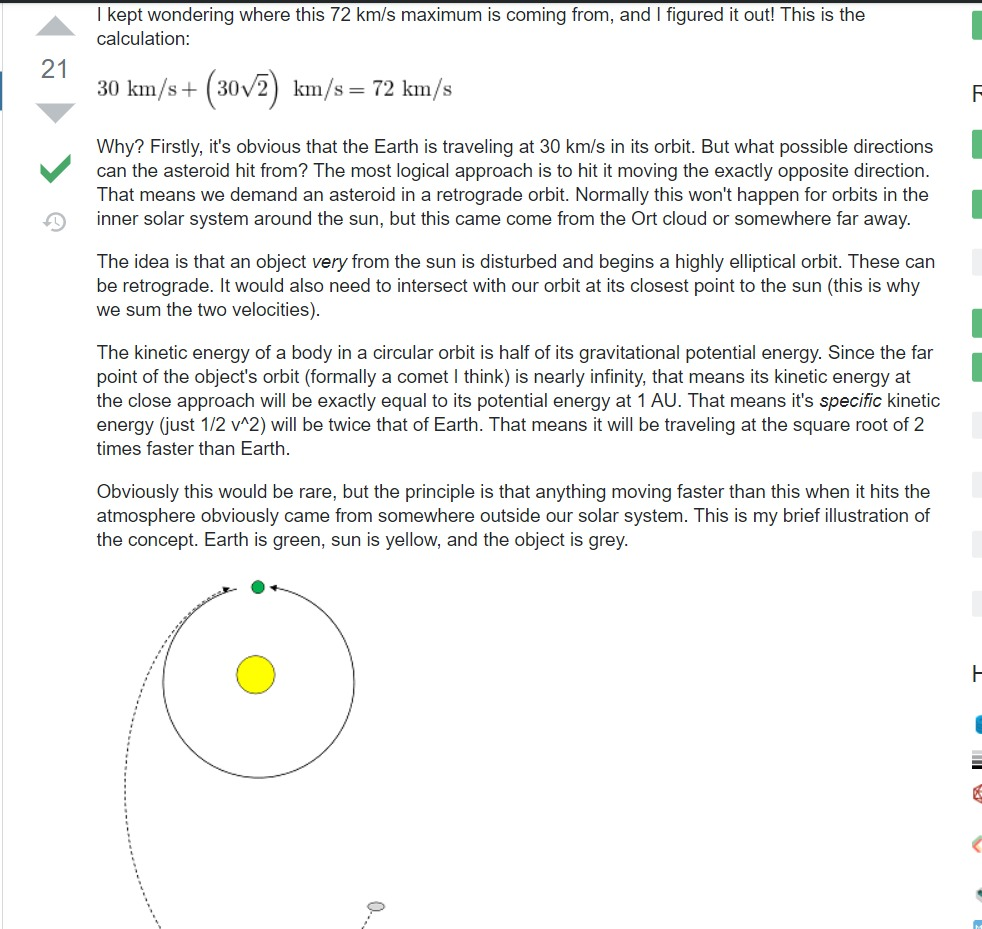
\includegraphics[width=0.7\linewidth]{pics/1b}
	\caption{}
	\label{fig:1b}
\end{figure}


VMin is 0: same velocity as the earth.

ii)E 1MT TNT $ = 4.5\e{15}$. $E = m \epsilon = m v_{E,C}^2 /2$. $m = \frac{2E}{v^2} =    \frac{24.5\e{15}}{(72000)^2} = 17372.98 tons$ (according to wikipedia, NASA estimates the mass as 10000 tons). Minimum mass: 0.


\textbf{(c)} i)There were many straw bodies in the early history of the solar system: early bombardment era. The frequency dropped off rapidly during the first billion and a half years to a roughly constant cratering flux during the past 3 Gyr. However, crater removal (e.g., because of active volcanism) can be a problem in this estimations. If a body is saturated with craters, it is ~4.5 Gyr old. If not, for example when the Moon was flooded with lava, craters dissapeared. (Section 6.4 of the book). ii) Figure 6.33 d and e of the book: Earth 1 to 100 Myr. Mars mostly 100 Myr - 1 Gyr



\textbf{(d)} i) There is a tidal bulge due to the Moon's attraction, but because of friction and other factors, this bulge generates a force with the Moon which generates a torque opposed to the rotation of the Earth. Thus, the Earth day has been getting slower and slower about 0.0016 seconds by year. Nicely explained in \url{https://www.astronomynotes.com/gravappl/s10.htm} ii) There are three dissipation phenomena: power needed to move the Moon to a higher orbit, dissipation of the rotational energy of the Earth and slowdown of the lunar eigen-rotation.





